\documentclass[12pt]{article}

\usepackage[utf8]{inputenc}
\usepackage{amsmath}
\usepackage{graphicx}
\usepackage{titlesec}
\usepackage{tcolorbox}
\usepackage{titling}
\usepackage{circuitikz}
\usepackage{enumitem}
\usepackage{wrapfig}
\usepackage{float}
\usepackage{pgfplots}
\usepackage{hyperref}
\usepackage{tikz}
\usepackage{amsmath}
\usetikzlibrary{patterns}
\pgfplotsset{compat=1.18}

\title{\bfseries Laborator Electricitate 4}
\author{Sîrghe Matei}
\date{\today}

\titleformat{\section}
  {\normalfont\Large\bfseries}{\thesection}{1em}{}

\begin{document}

\maketitle

\section{Problemă Seminar}
O cantitate de sarcină Q este distribuită sub formă de strat subțire sferic a=raza sferei. De-a lungul unui diametr al acestei sfere, se plimbă un corp punctiform cu sarcină q.Calculați forța cu care acționează sarcina Q asupra corpului punctiform cu sarcina q.

\subsection{Coordonate polare și aria de pe o sferă}

\begin{figure}[H]
    \centering
    \noindent
    \begin{minipage}{0.45\textwidth}
        \centering
        \begin{tikzpicture}[scale=0.75]
            \draw (0,0) circle (2cm);
            \draw (0,0) ellipse (2cm and 1cm);
            \draw[->] (-2,-2) -- (2,2) node[right] {$\vec{z}$};
            \draw[->] (-4,0) -- (4,0) node[right] {$\vec{x}$};
            \draw[->] (0,-4) -- (0,4) node[right] {$\vec{y}$};
        \end{tikzpicture}
        \caption{Cerc, elipsă și vectori}
        \label{fig:circle_ellipse_vectors}
    \end{minipage}
    \hfill
    \begin{minipage}{0.45\textwidth}
        \centering
        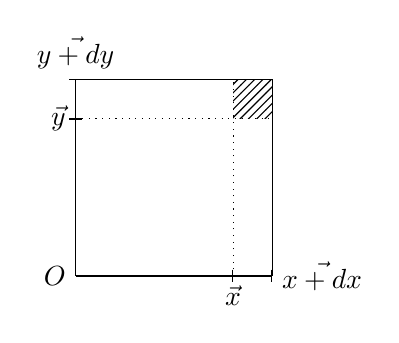
\begin{tikzpicture}
            \draw[-] (0,0) -- (0,0)node[anchor=east] {$O$};
            \draw[-|] (0,0) -- (2,0) node[anchor=north] {$\vec{x}$};
            \draw[-|] (2,0) -- (2.5,0) node[anchor=west] {$\vec{x+dx}$};
            \draw[-|] (0,0) -- (0,2) node[anchor=east] {$\vec{y}$};
            \draw[-|] (0,2) -- (0,2.5) node[anchor=south] {$\vec{y+dy}$};

            \fill[pattern=north east lines] (2,2) rectangle (2.5,2.5);
            \draw[dotted] (0,2) -- (2.5,2) {};
            \draw[dotted] (2,0) -- (2,2.5) {};
            \draw[-] (0,2.5) -- (2.5,2.5) {};
            \draw[-] (2.5,0) -- (2.5,2.5) {};
        \end{tikzpicture}
        \caption{Coordonate Carteziene}
        \label{fig:vectors_in_plane}
    \end{minipage}
\end{figure}

\begin{figure}[H]
    \centering
    \noindent
    \begin{minipage}{0.45\textwidth}
        \centering
        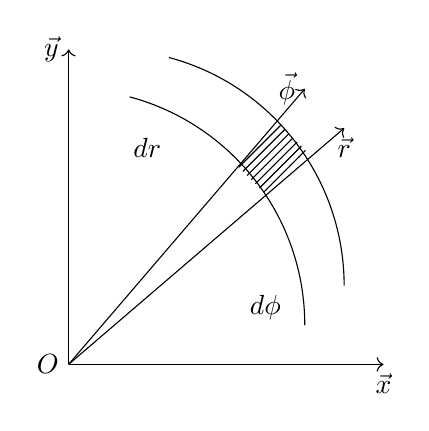
\begin{tikzpicture}
            \draw[-] (0,0) -- (0,0)node[anchor=east] {$O$};
            \draw[->] (0,0) -- (4,0) node[anchor=north] {$\vec{x}$};
            \draw[->] (0,0) -- (0,4) node[anchor=east] {$\vec{y}$};
            \draw (3,0.5) arc[start angle=0, end angle=75, radius=3cm];
            \draw (3.5,1) arc[start angle=0, end angle=75, radius=3cm];

            \draw[->] (0,0) -- (3.5,3) node[anchor=north] {$\vec{r}$};
            \draw[->] (0,0) -- (3,3.5) node[anchor=east] {$\vec{\phi}$};

            \draw (2.5,1) node[anchor=north] {$d\phi$};
            \draw (1,3) node[anchor=north] {$dr$};

            \fill[pattern=north east lines, rotate=45] (3.30,-0.25) rectangle (4.05,0.25);
        \end{tikzpicture}
        \caption{Coordonate Polare}
        \label{fig:vectors_in_plane}
    \end{minipage}
    \hfill
    \begin{minipage}{0.45\textwidth}
        \centering
        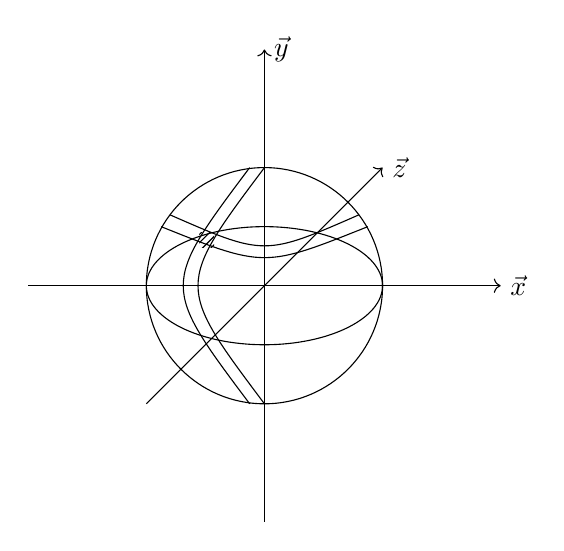
\begin{tikzpicture}[scale=0.75]
            \draw (0,0) circle (2cm);
            \draw (0,0) ellipse (2cm and 1cm);
            \draw[->] (-2,-2) -- (2,2) node[right] {$\vec{z}$};
            \draw[->] (-4,0) -- (4,0) node[right] {$\vec{x}$};
            \draw[->] (0,-4) -- (0,4) node[right] {$\vec{y}$};

            \draw (0,2) .. controls (-1.5,0) .. (0,-2);
            \draw (-0.25,2) .. controls (-1.75,0) .. (-0.25,-2);

            \draw (-1.6,1.2) .. controls (0,0.5) .. (1.6,1.2);
            \draw (-1.75,1) .. controls (0,0.3) .. (1.75,1);

            \fill[pattern=north east lines] (-1.1,0.9) rectangle (-0.85,0.65);
        \end{tikzpicture}
        \caption{Arie de pe sferă}
        \label{fig:circle_ellipse_vectors}
    \end{minipage}
\end{figure}

\subsection{Formule Matematice}

\begin{equation}
    dS=r dr d\phi \hspace{2cm} \phi \in [0,2\pi]\\
\end{equation}

\begin{equation}
 (x,y,z) \longrightarrow (r,\theta,\phi) \hspace{2cm} \theta \in [0,\pi]\\
\end{equation}

\begin{equation}
    \begin{cases}
        x = r \sin(\theta) \cos(\phi) \\
        y = r \sin(\theta) \sin(\phi) \hspace{2cm} x,y,z \in [-r,r] \\
        z = r \cos(\theta)
    \end{cases}
\end{equation}

\begin{equation}
    \begin{cases}
        L_{1} = rsin(\theta)d\phi \\
        L_{2} = rd\theta\\
        dS=r^{2}sin(\theta)d\theta d\phi
    \end{cases}
\end{equation}

\subsection{Simplificare Integrala dublă}

\begin{equation}
    \sum_{i=1}^{2}\sum_{j=1}^{3}a_{i}b_{j} = \sum_{i=1}^{2}(a_{i}b_{1}+a_{i}b_{2}+a_{i}b_{3}) = (a_{1}+a_{2})(b_{1}+b_{2}+b_{3})=(\sum_{i=1}^{2}a_{i})(\sum_{j=1}^{3}b_{j}) = \sum_{i=1}^{2}\sum_{j=1}^{3}a_{i}b_{j}
\end{equation}
\begin{equation}
    \implies \int_{a}^{b} \int_{a}^{b} f(x)f(y) \,\, = \int_{a}^{b} f(x) \, \int_{a}^{b} f(y) \,
\end{equation}

\subsection{Rezolvare Problemă}

\begin{figure}[H]
    \centering
    \noindent
    \begin{center}
        \centering
        \begin{tikzpicture}[scale=0.75]
            \draw (0,0) circle (2cm);
            \draw[->] (0,0) -- (1,0.5) node[right] {${r}^{'}$};
            \draw[->] (1,0.5) -- (0,3) node[left] {${r}$};
            \draw[->] (0,0) -- (-3,-3) node[right] {${x}$};
            \draw[->] (0,0) -- (4,0) node[right] {${z}$};
            \draw[->] (0,0) -- (0,4) node[right] {${y}$};

            \draw (0.25,3) node[right] {$q$};
            \draw (2,0.5) node[right] {$dQ_{'}$};
            \draw (0,-0.5) node[right] {$O$};
            \draw (-2,0) node[left] {$Q$};
        \end{tikzpicture}
        \caption{Schemă problemă}
        \label{fig:circle_ellipse_vectors}
    \end{center}
    \hfill
\end{figure}

\begin{equation}
    d\vec{F} = k \frac{ q dQ_{'} }{ \left| \vec{r} - \vec{r^{'}} \right|^{3} } ( \vec{r} - \vec{r^{'}} )\\
\end{equation}

\begin{equation}
    \begin{cases}
        Q     ............ 4\pi a^{2}\\
        dQ^{'}............ dS^{'} \\
        \implies dQ^{'} = \frac{Q dS^{'}}{4\pi a^{2}}
    \end{cases}
\end{equation}

\begin{equation}
    \begin{cases}
        \vec{r} - \vec{r^{'}}(-x^{'},-y^{'},z-z^{'})\\
        \vec{r} - \vec{r^{'}} = -x^{'}\vec{i} - y^{'}\vec{j} + (z-z^{'})\vec{k}\\
        \left| \vec{r} - \vec{r^{'}} \right| = \sqrt{x^{'2} + y^{'2} + (z-z^{'})^{2}}
    \end{cases}
\end{equation}
\begin{equation}
d\vec{F} = k \frac{ Q\frac{ dS^{'} }{ 4\pi a^{2} }q }{ {\sqrt{x^{'2} + y^{'2} + (z-z^{'})^{2}}}^{3} } (-x^{'}\vec{i} - y^{'}\vec{j} + (z-z^{'})\vec{k})\\
\end{equation}
\begin{equation}
= \frac{ kQq }{ 4\pi a^{2} } \frac{ dS^{'} }{ {{x^{'2} + y^{'2} + (z-z^{'})^{2}}}^{\frac{3}{2}} } (-x^{'}\vec{i} - y^{'}\vec{j} + (z-z^{'})\vec{k})\\
\end{equation}

\begin{equation}
    \begin{cases}
        dF_{x} = \frac{ kQq }{ 4\pi a^{2} } \frac{ dS^{'}(-x^{'}) }{ {(x^{'2} + y^{'2} + (z-z^{'})^{2})}^{\frac{3}{2}} }\\
        dF_{y} = \frac{ kQq }{ 4\pi a^{2} } \frac{ dS^{'}(-y^{'}) }{ {(x^{'2} + y^{'2} + (z-z^{'})^{2})}^{\frac{3}{2}} }\\
        dF_{z} = \frac{ kQq }{ 4\pi a^{2} } \frac{ dS^{'}(-z^{'}) }{ {(x^{'2} + y^{'2} + (z-z^{'})^{2})}^{\frac{3}{2}} }
    \end{cases}
\end{equation}

\begin{equation}
    \begin{cases}
        F_{x} = \frac{ kQq }{ 4\pi a^{2} }\int_{}^{} \frac{ dS^{'}(-x^{'}) }{ {(x^{'2} + y^{'2} + (z-z^{'})^{2})}^{\frac{3}{2}} }\\
        F_{y} = \frac{ kQq }{ 4\pi a^{2} }\int_{}^{} \frac{ dS^{'}(-y^{'}) }{ {(x^{'2} + y^{'2} + (z-z^{'})^{2})}^{\frac{3}{2}} }\\
        F_{z} = \frac{ kQq }{ 4\pi a^{2} }\int_{}^{} \frac{ dS^{'}(-z^{'}) }{ {(x^{'2} + y^{'2} + (z-z^{'})^{2})}^{\frac{3}{2}} }
    \end{cases}
\end{equation}

\begin{equation}
    \begin{cases}
        x^{'}=a sin\theta cos\phi\\
        y^{'}=a sin\theta sin\phi\\
        z^{'}=a cos\theta
    \end{cases}
\end{equation}

$ \implies {(x^{'2}+y^{'2}+ {(z-z^{'})}^{2})}^{\frac{3}{2}} = {( a^{2} sin^{2}\theta cos^{2}\phi + a^{2}sin^{2}\theta sin^{2}\phi + {(z- a cos\theta)}^{2} )}^{\frac{3}{2}} $
$ = {( a^{2} sin^{2} \theta + {( z - a cos\theta )}^{2} )}^{\frac{3}{2}} $
$ ={( a^{2} sin^{2}\theta + z^{2} + a^{2} cos^{2}\theta - 2a + cos\theta )}^{\frac{3}{2}} $\\
$ = {( a^{2} + z^{2} -2a + cos\theta )}^{\frac{3}{2}} = a^{3} {( 1+ {(\frac{z}{a})}^{2} - 2 \frac{z}{a} cos\theta )}^{\frac{3}{2}}$\\
$ = a^{3} \left( \left( \frac{z}{a} \right)^{2} - \cos\theta \frac{z}{a} + 1 \right) ^ {\frac{3}{2}} \quad \text{notăm} \quad \frac{z}{a} = m $\\
$ \implies a^{3} {(m^{2} - cos\theta m +1 )}^{\frac{3}{2}} $

\begin{equation}
    \begin{cases}
        F_{x} = \frac{ kQq }{ 4\pi a^{2} }\int_{0}^{\pi} \int_{0}^{2\pi} \frac{ a^{2} sin\theta d\theta d\phi (-asin\theta cos\phi) }{ a^{3} {(1 + m^{2} - 2mcos\theta)}^{\frac{3}{2}} }\\ \\

        F_{y} = \frac{ kQq }{ 4\pi a^{2} }\int_{0}^{\pi} \int_{0}^{2\pi} \frac{ a^{2} sin\theta d\theta d\phi (-asin\theta sin\phi) }{ a^{3} {(1 + m^{2} - 2mcos\theta)}^{\frac{3}{2}} }\\ \\

        F_{z} = \frac{ kQq }{ 4\pi a^{2} }\int_{0}^{\pi} \int_{0}^{2\pi} \frac{ a^{2} sin\theta d\theta d\phi (z - acos\theta) }{ a^{3} {(1 + m^{2} - 2mcos\theta)}^{\frac{3}{2}} }\\

    \end{cases}
\end{equation}

\begin{equation}
    \begin{cases}
        F_{x} = \frac{ kQq }{ 4\pi a^{2} }\int_{0}^{\pi} \int_{0}^{2\pi} \frac{ sin^{2}\theta d \theta (-cos\phi d \phi) }{ {(1+m^{2} -2m cos\theta)}^{\frac{3}{2}} }\\ \\

        F_{y} = \frac{ kQq }{ 4\pi a^{2} }\int_{0}^{\pi} \int_{0}^{2\pi} \frac{ sin^{2}\theta d \theta (-sin\phi d \phi) }{ {(1+m^{2} -2m cos\theta)}^{\frac{3}{2}} }\\ \\

        F_{z} = \frac{ kQq }{ 4\pi a^{2} }\int_{0}^{\pi} \int_{0}^{2\pi} \frac{ sin^{2}\theta d \theta d \phi (m - cos\theta) }{ {(1+m^{2} -2m cos\theta)}^{\frac{3}{2}} }\\

    \end{cases}
\end{equation}

\begin{equation}
    \begin{cases}
        F_{x} = \frac{ kQq }{ 4\pi a^{2} }\int_{0}^{\pi} \frac{ sin^{2}\theta d \theta }{ {(1+m^{2} -2m cos\theta)}^{\frac{3}{2}} } \int_{0}^{2\pi} (-cos\phi d \phi) = 0 \\ \\

        F_{y} = \frac{ kQq }{ 4\pi a^{2} }\int_{0}^{\pi} \frac{ sin^{2}\theta d \theta }{ {(1+m^{2} -2m cos\theta)}^{\frac{3}{2}} } \int_{0}^{2\pi} (-sin\phi d \phi) = 0\\ \\

        F_{z} = \frac{ kQq }{ 4\pi a^{2} }\int_{0}^{\pi} \frac{ sin^{2}\theta d \theta (m - cos\theta) }{ {(1+m^{2} -2m cos\theta)}^{\frac{3}{2}} } \int_{0}^{2\pi} d \phi\\

    \end{cases}
\end{equation}

\begin{equation}
    \begin{cases}
        F_{x} = 0 \\ 
        F_{y} =  0\\ 
        F_{z} = \frac{ kQq }{ 2 a^{2} }\int_{0}^{\pi} \frac{ (m - cos\theta) sin\theta d \theta }{ {(1+m^{2} -2m cos\theta)}^{\frac{3}{2}} } d \theta\\

    \end{cases}
\end{equation}

\begin{equation}
    \implies F_{z} = \frac{ kQq }{ 2 a^{2} } \int_{-1}^{1} \frac{ (m - x) dx }{ {(1+m^{2} -2m x)}^{\frac{3}{2}} }\\
\end{equation}
\begin{equation}
    F_{z} = \frac{ kQq }{ 4m a^{2} } \int_{-1}^{1} \frac{ (-m^{2}-2mx) dx }{ {(1+m^{2} -2m x)}^{\frac{3}{2}} }\\
\end{equation}
\begin{equation}
    F_{z} = \frac{ kQq }{ 4m a^{2} } \int_{-1}^{1} \frac{ ( 1 + m^{2}-2mx+m^{2}-1 ) dx }{ {(1+m^{2} -2m x)}^{\frac{3}{2}} }\\
\end{equation}
\begin{equation}
    F_{z} = \frac{ kQq }{ 4m a^{2} } \int_{-1}^{1} \frac{ (m^{2}-2mx)dx }{ {(1+m^{2}-2mx)}^{\frac{3}{2}} } \int_{-1}^{1} \frac{ (m^{2} - 1)dx }{ {(1+m^{2}-2mx)}^{\frac{3}{2}}} \\
\end{equation}
\begin{equation}
    F_{z} = \frac{ kQq }{ 4m^{2} a^{2} } \int_{-1}^{1} {(1 + m^{2} -2mx)}^{-\frac{1}{2}} \int_{-1}^{1} {(1 + m^{2} -2mx)}^{-\frac{3}{2}} \\
\end{equation}
\begin{equation}
    F_{z} =- \frac{ kQq }{ 4m^{2} a^{2} } \left( \left| m - 1 \right| - \left| m + 1 \right| - \left( m^{2} - 1 \right) \left( \frac{1}{ \left| m - 1 \right| } - \frac{1}{ \left| m + 1 \right| } \right) \right)\\
\end{equation}

$ m=\frac{z}{a} ; m>1 \implies z > a$ deasupra mingii 

\begin{equation}
   \implies F_{z} =- \frac{ kQq }{ 4m^{2} a^{2} } \left(  m - 1  - ( m + 1)  - \left( m^{2} - 1 \right) \left( \frac{1}{  m - 1  } - \frac{1}{  m + 1  } \right) \right)\\
\end{equation}

\begin{equation}
    F_{z} =- \frac{ kQq }{ 4m^{2} a^{2} } \left(  -4\right) \\
\end{equation}

\begin{equation}
    F_{z} = \frac{ 4kQq }{ 4m^{2} a^{2} } = \frac{kQq}{m^{2}a^{2}}=\frac{kQq}{z^{2}} \\
\end{equation}

$ m=\frac{z}{a} ; m<1 \implies z < a$ în minge 

\begin{equation}
   \implies F_{z} =- \frac{ kQq }{ 4m^{2} a^{2} } \left(  1-m  - ( m + 1)  - \left( m^{2} - 1 \right) \left( \frac{1}{  1 - m  } - \frac{1}{  m + 1  } \right) \right)\\
\end{equation}

\begin{equation}
    F_{z} =- \frac{ kQq }{ 4m^{2} a^{2} } \left( 0m \right) \\
\end{equation}

\begin{equation}
    F_{z} = 0 \\
\end{equation}

\end{document}